% Dieser Text ist urheberrechtlich gesch�tzt
% Er stellt einen Auszug eines von mir erstellten Referates dar
% und darf nicht gewerblich genutzt werden
% die private bzw. Studiums bezogen Nutzung ist frei
% Januar 2006
% Autor: Sascha Frank
% Universit�t Freiburg
% www.informatik.uni-freiburg.de/~frank/
% www.namsu.de/


% \documentclass[handout]{beamer} % to remove transitions for printing
\documentclass{beamer}
\usetheme{Boadilla}
\usecolortheme{beaver}
\usepackage[english]{babel}
%\usepackage{german}

%\setbeamercolor{enumerate item}{ fg=red} % enumerate items red
\setbeamercolor{item projected}{bg=red}
\usepackage[export]{adjustbox}
\usepackage{graphicx}
\usepackage{subfigure}
\usepackage{booktabs}                      %% Befehle fuer besseres Tabellenlayout
\usepackage{color}
\definecolor{myred}{rgb}{0.8, 0.0, 0.0}
\definecolor{mygreen}{RGB}{0, 100, 0}
\setbeamercovered{highly dynamic}
\setbeamercolor{caption name}{fg=red}

\usepackage{bbding}

%\usepackage[usenames,dvipsnames,svgnames,table]{xcolor}

%\usepackage[skins,theorems]{tcolorbox}
%\tcbset{highlight math style={enhanced,
%    colframe=myred,colback=white,arc=0pt,boxrule=1pt}}

\usepackage{appendixnumberbeamer}

\newcounter{saveenumi}
\newcommand{\seti}{\setcounter{saveenumi}{\value{enumi}}}
\newcommand{\conti}{\setcounter{enumi}{\value{saveenumi}}}

\resetcounteronoverlays{saveenumi}


\makeatother
\setbeamertemplate{footline}
{
  \leavevmode%
  \hbox{%
    \begin{beamercolorbox}[wd=.4\paperwidth,ht=2.25ex,dp=1ex,center]{author in head/foot}%
      \usebeamerfont{author in head/foot}\insertshortauthor
    \end{beamercolorbox}%
    \begin{beamercolorbox}[wd=.6\paperwidth,ht=2.25ex,dp=1ex,center]{title in head/foot}%
      \usebeamerfont{title in head/foot}\insertshorttitle\hspace*{3em}
      \insertframenumber{} / \inserttotalframenumber\hspace*{1ex}
    \end{beamercolorbox}}%
  \vskip0pt%
}
\makeatletter
\setbeamertemplate{navigation symbols}{}


\begin{document}

\title{Some Words about Lab Reports}
%\author{Edgar Kellermann, Caterina Doglioni}
%\date{\today}
\date{FYSC12}
%\institute{Lund University}
%\logo{\includegraphics[scale=0.50]{pictures/Logo_Uni_Goettingen.pdf}}

\begin{frame}
  
\includegraphics[scale=0.20]{pictures/LundUniversity.png}
  \titlepage
\end{frame}

\begin{frame}
 \frametitle{Table of Contents}\tableofcontents
\end{frame}

\section{Content}
\begin{frame}
  \frametitle{The structure of a report }

  \begin{minipage}{0.39\linewidth}
    \begin{figure}[h]
      \centering
      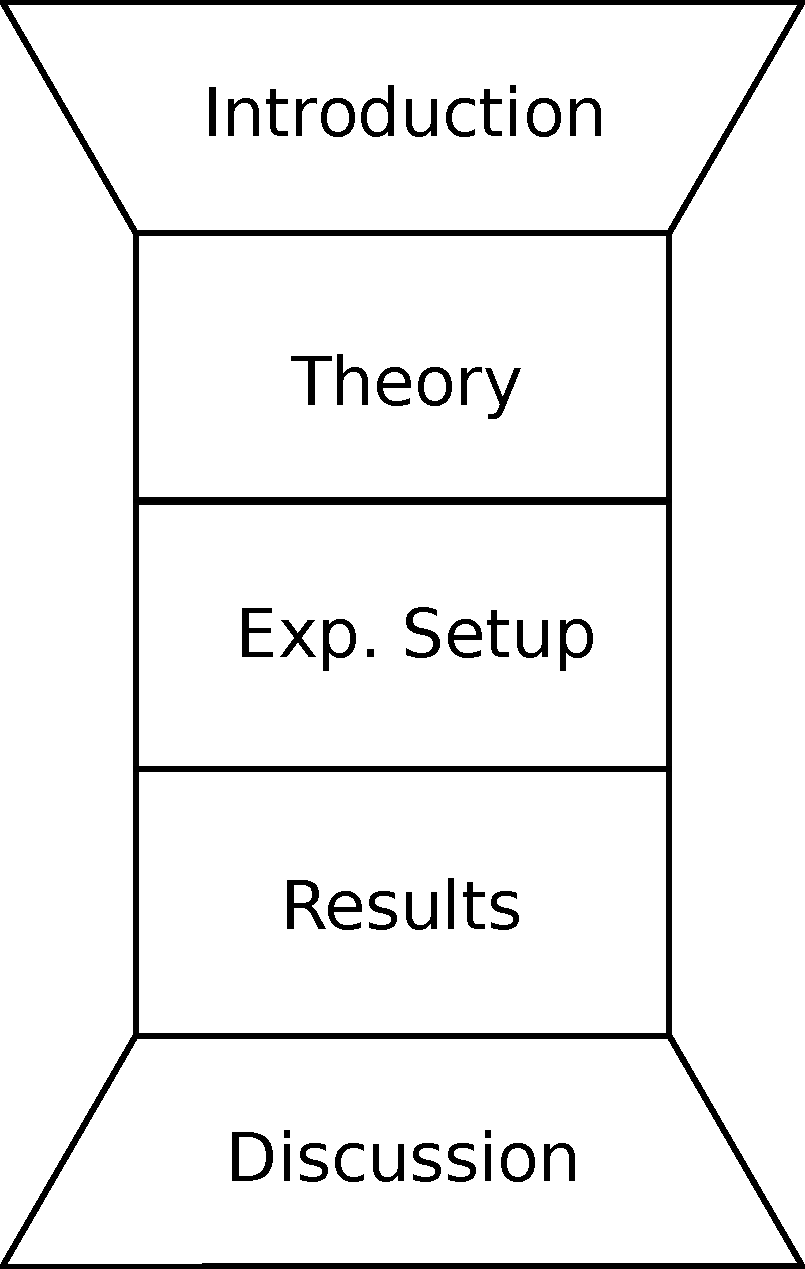
\includegraphics[scale=0.30]{pictures/structure.pdf}
      \caption{\small \color{blue} [Cargill, O'Connor, Writing
        Scientific Research Articles]]}
      \label{img:1}
    \end{figure}
  \end{minipage}%
  \begin{minipage}{0.59\linewidth}
    \vspace{-1.5cm}
    \begin{itemize}
    \item \textbf{Introduction}: pick up the reader from a broader field and
      pull him/her into your specific topic
      \vspace{2,5cm}
    \item \textbf{Results}: key driver of your report, here is the big
      message
    \item \textbf{Discussion}: Recapitulating what was done, go back
      to the broader field
    \end{itemize}
  \end{minipage}

\end{frame}

\begin{frame}
  \frametitle{Results}
  \begin{minipage}{0.39\linewidth}
    \begin{figure}[h]
      \centering
      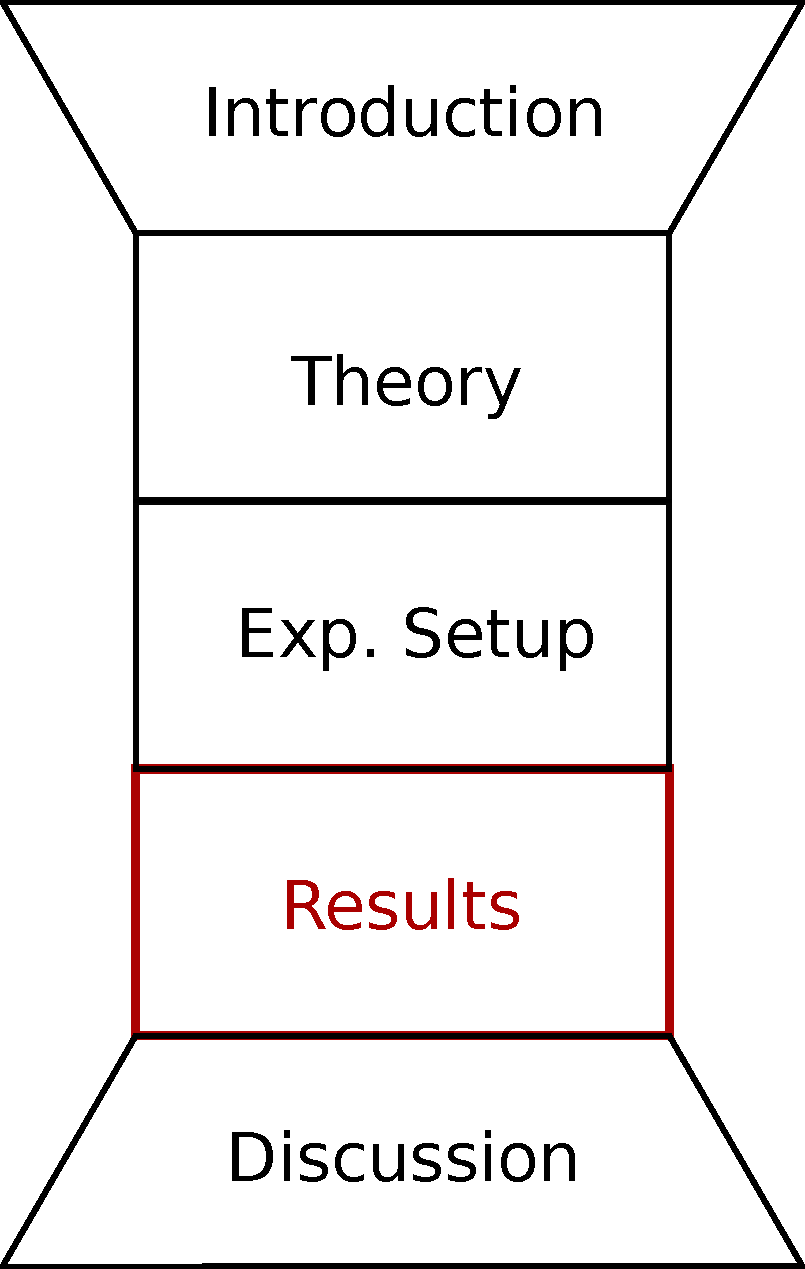
\includegraphics[scale=0.30]{pictures/structureResults.pdf}
      \caption{\small \color{blue} [Cargill, O'Connor, Writing
        Scientific Research Articles]]}
      \label{img:1}
    \end{figure}
  \end{minipage}%
  \begin{minipage}{0.59\linewidth}
    \vspace{-1cm}
    \begin{itemize}
    \item What did I measure and what are the \textbf{final results}
      of my experiment?
    \item How do I \textbf{illustrate} the results in an easy way?
      (Use figures and tables)
    \item What are the \textbf{statistical and systematic
        uncertainties} that I have to consider and how big are they?
    \end{itemize}
  \end{minipage}
\end{frame}

\begin{frame}
  \frametitle{Example for a Figure}

  \begin{figure}[h]
    \centering
    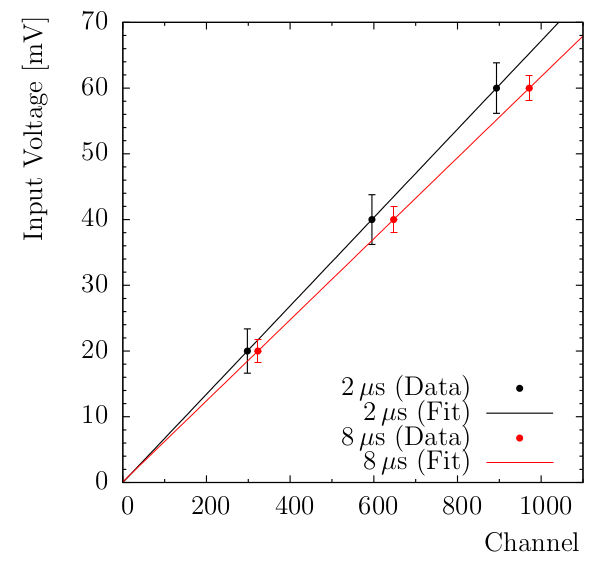
\includegraphics[scale=0.25]{pictures/Calibration.png}
    \caption{The input voltage over the measured channel used for the
      calibration of the preamplifier. The statistical error are given
      by the FWHM of a Gaussian fit.}
    \label{img:1}
  \end{figure}

  \textcolor{myred}{DON'T FORGET:} axis labels, units, complete legend, tics, range

\end{frame}

\begin{frame}
  \frametitle{Example for a Table}
  \begin{table}
    \centering
    \caption{The parameters of the $\chi^{2}$ fits for the shape times of
      2 and 8 $\mu$s.}
    \begin{tabular}{ccc}
      \hline
      shape time [$\mu$s] & intercept [$10^{-2}$ mV] & gradient [$10^{-2}$ mV/channel] \\
      \hline
      2 &  -0.82 $\pm$  0.08 & 6.7179 $\pm$ 0.0002 \\
      8 & 8.3 $\pm$ 0.9 & 6.1657 $\pm$ 0.0002 \\
      \hline
    \end{tabular}
    \label{tab:calibrationParameters}
  \end{table}
  \textbf{Every measured data has an error!}\\
  Two ways of illustrating errors:
  \begin{enumerate}
  \item 6.7179 $\pm$ 0.0002
  \item 6.7179(2)
  \end{enumerate}

\end{frame}

\begin{frame}
  \frametitle{Theory and Experimental Setup}
  \begin{minipage}{0.39\linewidth}
    \begin{figure}[h]
      \centering
      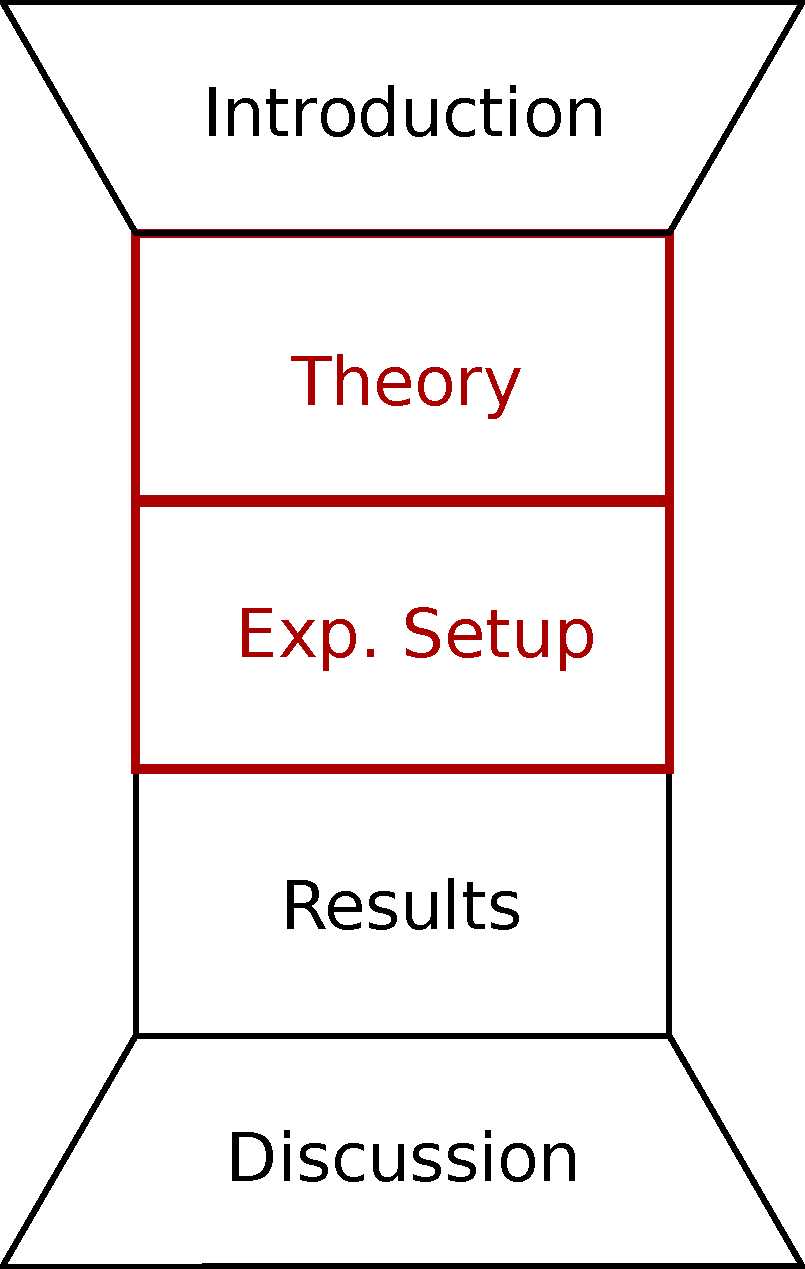
\includegraphics[scale=0.30]{pictures/structureTheorySetup.pdf}
      \caption{\small \color{blue} [Cargill, O'Connor, Writing
        Scientific Research Articles]]}
      \label{img:1}
    \end{figure}
  \end{minipage}%
  \begin{minipage}{0.59\linewidth}
    \vspace{-2cm}
    \textbf{Theory:}
 %   \vspace{-0.5cm}
    \begin{itemize}
    \item Which concepts (formulas, models, approximations) are
      essential and used in my \textbf{Results section}?
    \item For your own good, write only \textbf{1 page} of theory
      $\Rightarrow$ Use \textbf{references}!
    \end{itemize}
    \textbf{Experimental Setup:}
%    \vspace{-0.5cm}
    \begin{itemize}
    \item  What information is required to \textbf{redo} my experiment
      and \textbf{reproduce} my results?
    \end{itemize}
  \end{minipage}
\end{frame}


\begin{frame}
  \frametitle{Introduction and Discussion}
  \begin{minipage}{0.39\linewidth}
    \begin{figure}[h]
      \centering
      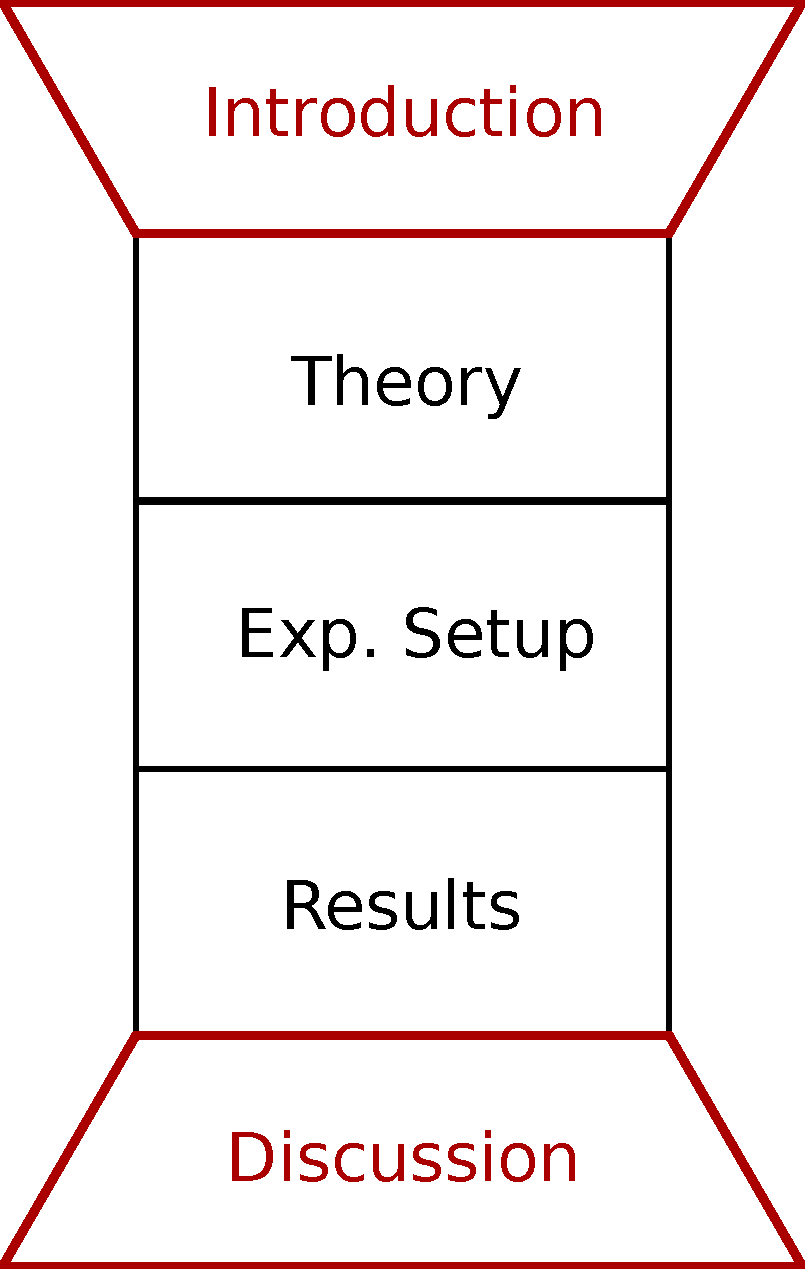
\includegraphics[scale=0.30]{pictures/structureIntroductionDiscussion.pdf}
      \caption{\small \color{blue} [Cargill, O'Connor, Writing
        Scientific Research Articles]]}
      \label{img:1}
    \end{figure}
  \end{minipage}%
  \begin{minipage}{0.59\linewidth}
    \textbf{Introduction:}
    % \vspace{-0.5cm}
    \begin{itemize}
    \item Motivate your work: Why do we do this experiment?
    \item Why in this specific way?
    \item What do I expect/ hope to see?
    \end{itemize}
    \textbf{Discussion:}
    % \vspace{-0.5cm}
    \begin{itemize}
    \item Summarise your results: What is the \textbf{take-away message}?
    \item Discuss effects and amount of systematic uncertainties
    \item How did these results contribute to our knowledge from a
      broader point of view?
    \end{itemize}
  \end{minipage}
\end{frame}

\begin{frame}
  \frametitle{Nearly finished but don't forget:}

  \begin{minipage}{0.39\linewidth}
    \begin{figure}[h]
      \centering
      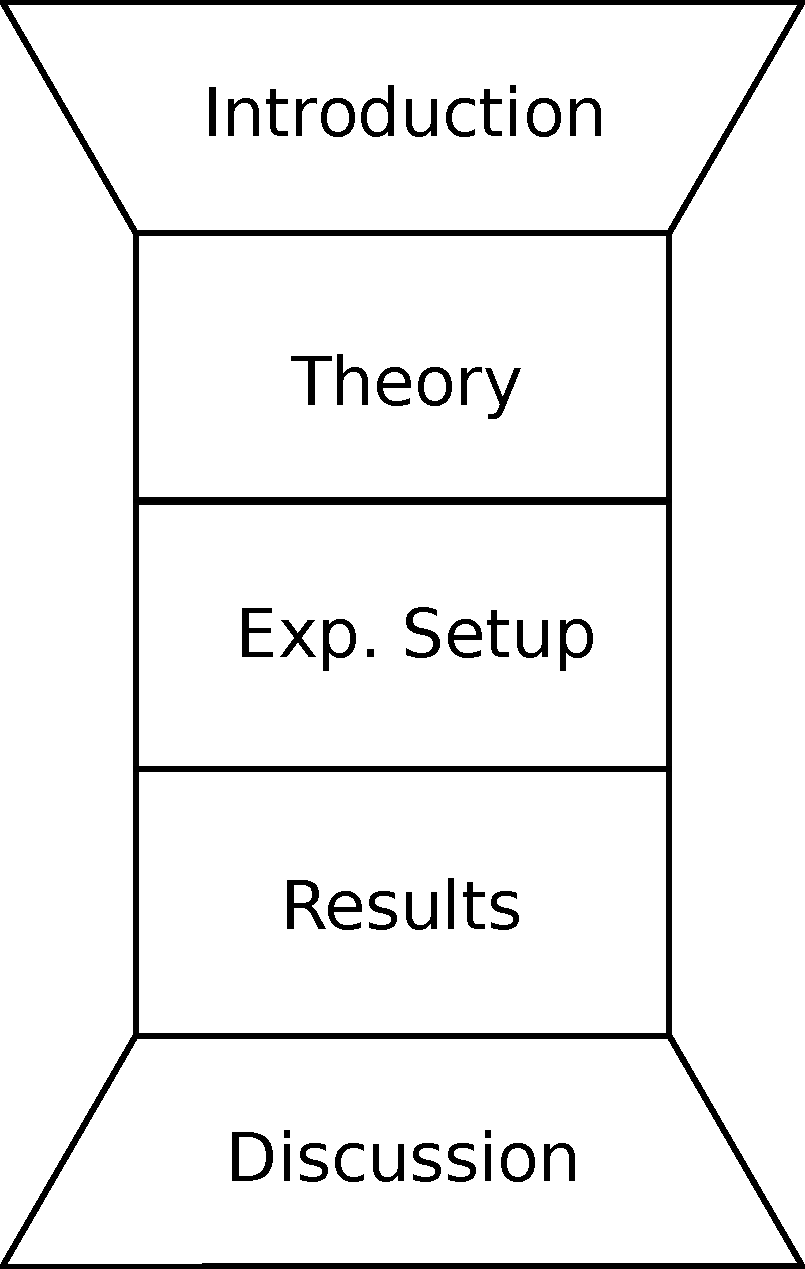
\includegraphics[scale=0.30]{pictures/structure.pdf}
      \caption{\small \color{blue} [Cargill, O'Connor, Writing
        Scientific Research Articles]]}
      \label{img:1}
    \end{figure}
  \end{minipage}%
  \begin{minipage}{0.59\linewidth}
    \vspace{-1.5cm}
    \textbf{Read you own report again and check:}
    \begin{itemize}
      \item Do I have a continuous text flow? Do I introduce every
        section and make clear what I am talking about? Do I use
        complete, grammatically correct sentences?
      \item Is any physicist from outside able to
        understand my report?
      \item Can anyone reproduce your measurements?
      \item \textbf{tip:} Read your report from the back to the front! You
        will find a lot of mistakes that you have not recognised before!
    \end{itemize}
  \end{minipage}

\end{frame}

\section{Examples of things NOT to do}

\begin{frame}
  \frametitle{(Bad) Example 1:}
  \begin{figure}[h]
    \centering
    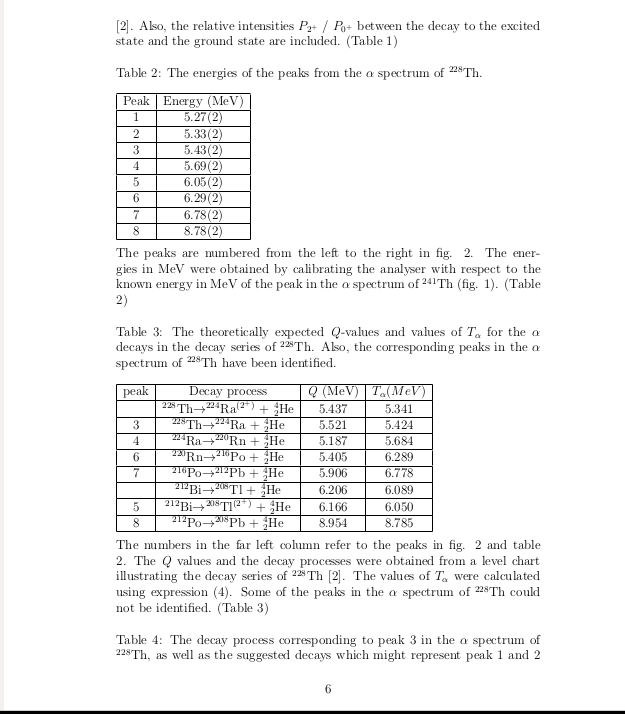
\includegraphics[scale=0.25]{pictures/DONOT3.png}
  \end{figure}
\uncover<2>{\small{\textcolor{myred}{\XSolidBrush tables not centered}}\qquad}
\end{frame}

\begin{frame}
  \frametitle{(Bad) Example 2:}
  \begin{figure}[h]
    \centering
    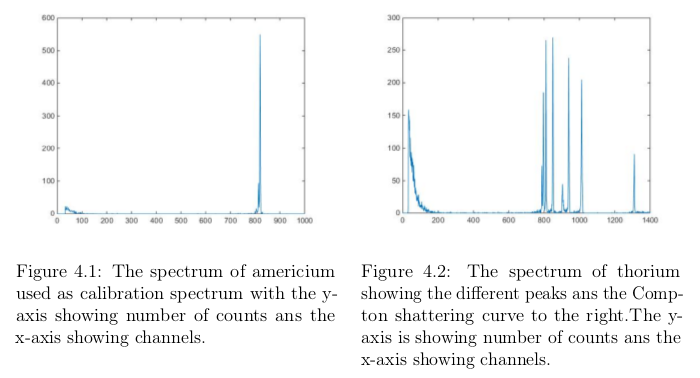
\includegraphics[scale=0.40]{pictures/DONOT1.png}
  \end{figure}
\uncover<2->{\small{\textcolor{myred}{\XSolidBrush no axis
      labels}}\qquad}
\uncover<2->{\small{\textcolor{myred}{\XSolidBrush no units}}\qquad}
\uncover<3>{\small{\textcolor{myred}{\XSolidBrush not zoomed in}}
\begin{center}
  \color{myred}{DO NOT TRY THIS AT HOME!}
\end{center}
}
\end{frame}

\begin{frame}
  \frametitle{(Bad) Example 2:}
  \begin{figure}[h]
    \centering
    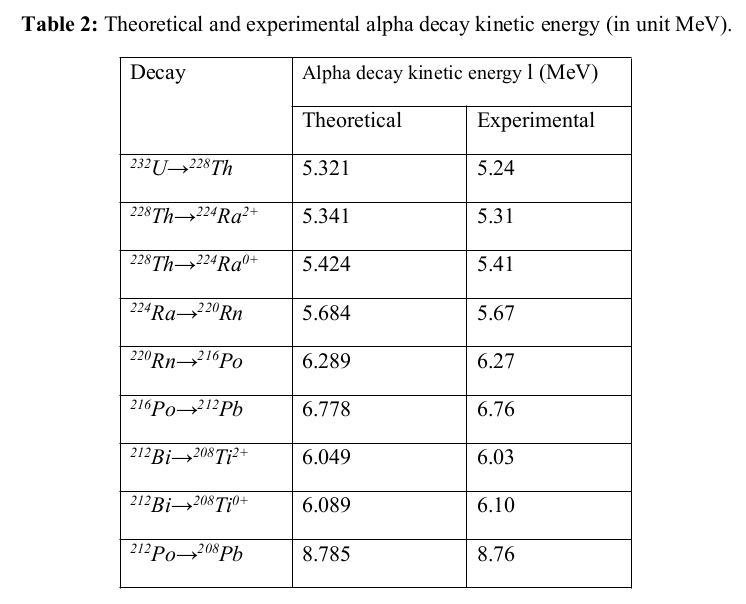
\includegraphics[scale=0.30]{pictures/DONOT2.png}
  \end{figure}
\uncover<2->{\small{\textcolor{myred}{\XSolidBrush inconsistent digits}} \qquad}
\uncover<3->{\small{\textcolor{myred}{\XSolidBrush no uncertainties}}
  \qquad}
\uncover<4>{\small{\textcolor{myred}{\XSolidBrush {\it Theoretical/Tabulated}?~Refs?}} }
\end{frame}

 \begin{frame}
   \frametitle{Rule of Thumb}
   \begin{enumerate}

   \item Never notate measured values \textbf{without} errors!
     \begin{align}
       m = (100.0 \pm 0.2) \text{g} \quad
       \text{\textbf{or}} \quad  m &= 100.0(2) \text{g}
     \end{align}
   \item Always round errors \textbf{up} if you need to round. \\
 %    e.g. $\Delta x = 0.783 \Rightarrow \Delta x \approx 0.8$
     \vspace{2mm}
   \item Notate the mean value with the \textbf{same number of digits}
     as the error
     \textcolor{myred}{$m = (99.98432 \pm 0.2) \text{g}$\quad\XSolidBrush}\\
     \textcolor{mygreen}{$m = (100.0 \pm 0.2) \text{g}$\quad\quad\quad\Checkmark}
   \end{enumerate}
 \end{frame}

 \begin{frame}
   \frametitle{Error Propagation (good) example}
 %  general formula of error propagation for a function $f(a,b,c,...)$:
 %  \begin{align}
 %    \sigma_{f}^{2} = \left( \frac{\partial f}{\partial a} \right)^{2}
 %    \sigma_{a}^{2} +  \left( \frac{\partial f}{\partial b} \right)^{2}
 %    \sigma_{b}^{2} +  \left( \frac{\partial f}{\partial c} \right)^{2}
 %    \sigma_{c}^{2} + ...
 %  \end{align}
   \textbf{Example:} How big is the error of the spring constant $D$?
   \\
   \vspace{0.5cm}
   $\quad \quad D = \textcolor{blue}{m} \cdot \textcolor{magenta}{\omega^{2}}, \quad \textcolor{blue}{m = (99.9 \pm 0.2)\;
   \text{g}}, \quad \textcolor{magenta}{\omega = (0.6 \pm 0.1)\; \text{s}^{-1}} $ \\
   \quad \quad (\textcolor{blue}{$m$} and \textcolor{magenta}{$\omega$} independent)
   \begin{align*}
     \sigma_{D}^{2} &= \left( \frac{\partial
                      D(m,\omega)}{\textcolor{blue}{\partial m}} \right)^{2}
     \textcolor{blue}{\sigma_{m}^{2}} +  \left( \frac{\partial
                      D(m,\omega)}{\textcolor{magenta}{\partial \omega}} \right)^{2}
     \textcolor{magenta}{\sigma_{\omega}^{2}} \\
 %    &= (\omega^{2})^{2} \sigma_{m}^{2} + (2 \omega m)^{2}
 %    \sigma_{\omega}^{2}\\
     &= \omega^{4} \sigma^{2}_{m} + 4 \omega^{2}m^{2}
     \sigma^{2}_{\omega} \\
     \sigma_{D} &\approx 11.99 \; \frac{\text{g}}{\text{s}^{2}} \quad (\text{round up!})
   \end{align*}
For a final value of
   \begin{center}
     \begin{equation*}
       D = \left(36 \pm 12\right) \frac{g}{s^2}
     \end{equation*}
   \end{center}
 \end{frame}

 \begin{frame}
   \frametitle{Additional material}
   \begin{itemize}
   \item Do not forget to check the ``FYSC12 Pro Forma Lab Report''
     guide (even with \LaTeX source).
   \item Also, use the ``Practical Introduction Error Analysis'' as
     guidance.
   \end{itemize}
 \end{frame}

\section{Deadline and Corrections}
\begin{frame}
  \frametitle{Deadline and Corrections}
  \begin{itemize}
  \item You are allowed to work \textbf{in pairs of two}!
  \item Submit the finished report via the course webpage!\\
    \pause
  \normalsize \item \textbf{Deadline for submitting the report}:\\
    \textbf{10} working days after your lab.
    \begin{itemize}
    \item in case you hand it in too late: Maximum grade can only be
      50 \% (pass)
    \end{itemize}\pause
  \item Corrections by the supervisor in about 10 working days. Reports
    will be graded from 0 to 100 \%.
    \begin{itemize}\pause
    \item \textbf{Case 1}: grade $\geq$ 50\% you \color{mygreen}{passed}
      \color{black}, well done! \pause
    \item \textbf{Case 2}: grade $<$ 50\% you \color{myred}{failed}...\\
      \color{black} Your supervisor might hand you back your report and
      ask you for corrections. Your \textbf{final grade} will be the
      average of your first and second report!
    \end{itemize}
  \item 2nd hand-ins need to be submitted within 5 working days counting from the day the corrected report was returned.
  \end{itemize}
\end{frame}

\begin{frame}
  \frametitle{That's it!}
  \begin{center}
    \Huge\color{myred}{Questions?}
  \end{center}
\end{frame}

 %%% TODO:
 % 12g mit zwei mehr Stellen
 % Pic von Webseite am Schluss (roter Kasten)
 % Least square method

\end{document}







%-- how to structure a report
%-- figures
%-- references
%--

%\begin{frame}
%  \frametitle{Update of my work}
%
%  \begin{enumerate}
%  \item Generate MC NTuples (as an example) \textcolor{mygreen}{[DONE]}
%  \item Understand Brian's \textbf{Mass Binning} Code
%    \textcolor{orange}{[WORK IN PROGRESS]}  \\ (jet
%    resolution calculation included)
%  \item Adapt to \textbf{trigger jets} \\
%    \textcolor{orange}{Just replacing reco with trigger jets?}
%  \item Use trigger jets NTuples
%  \end{enumerate}
%
%  \begin{minipage}{0.49\linewidth}
%    \begin{figure}[h]
%      \centering
%      \includegraphics[scale=0.25]{pictures/2_resolutionBin_10.pdf}
%      \caption{Response plot for one bin.}
%      \label{img:1}
%    \end{figure}
%  \end{minipage}%
%  \begin{minipage}{0.49\linewidth}
%    \begin{figure}[h]
%      \centering
%      \includegraphics[scale=0.25]{pictures/2_resolution.pdf}
%      \caption{Jet resolution for $m_{jj}$}
%      \label{img:1}
%    \end{figure}
%  \end{minipage}
%\end{frame}


 \begin{frame}
   \frametitle{Least Square Method}
   \textbf{How do I fit the a line to my measured data?}
   \begin{minipage}{0.49\linewidth}
     \begin{align*}
       f(x) = m(x_{i},\sigma_{i}) \cdot x + n(x_{i},\sigma_{i})
     \end{align*}
     Use \textbf{least-square fitting} ($\chi^{2}$ method/ linear
     regression):
     minimise the value $\chi^{2}$:
     \begin{align*}
       \chi^{2} = \sum_{i} \frac{1}{\sigma_{i}} &(y_{i} - m - n \cdot
       x_{i})^{2}\\
       \Rightarrow m(x_{i},\sigma_{i}) &= ... , \\
       n(x_{i},\sigma_{i}) &= ...
     \end{align*}
   \end{minipage}%
   \begin{minipage}{0.49\linewidth}
     \begin{figure}[h]
       \centering
       %\includegraphics[scale=0.45]{pictures/visko.pdf}
       \caption{fitting a  line to the measured data}
       \label{img:1}
     \end{figure}
   \end{minipage}
 \end{frame}

 \begin{frame}
   \frametitle{More Informations on the Web}

     \begin{figure}[h]
       \centering
       %\includegraphics[scale=0.40]{pictures/screenshot.png}
       \label{img:1}
     \end{figure}

 \end{frame}

 \begin{frame}
   \frametitle{More Informations on the Web}

   \begin{figure}[h]
     \centering
     %\includegraphics[scale=0.30,frame]{pictures/screenshot2.png}
     \label{img:1}
   \end{figure}

 \end{frame}
